%
% File acl2020.tex
%
%% Based on the style files for ACL 2020, which were
%% Based on the style files for ACL 2018, NAACL 2018/19, which were
%% Based on the style files for ACL-2015, with some improvements
%%  taken from the NAACL-2016 style
%% Based on the style files for ACL-2014, which were, in turn,
%% based on ACL-2013, ACL-2012, ACL-2011, ACL-2010, ACL-IJCNLP-2009,
%% EACL-2009, IJCNLP-2008...
%% Based on the style files for EACL 2006 by 
%%e.agirre@ehu.es or Sergi.Balari@uab.es
%% and that of ACL08 by Joakim Nivre and Noah Smith


\documentclass[11pt,a4paper]{article}
\usepackage[hyperref]{acl2020}
\usepackage{times}
\usepackage{latexsym}
\renewcommand{\UrlFont}{\ttfamily\small}
\renewcommand{\arraystretch}{1.2}
\usepackage{hyperref}
\usepackage{graphicx}
\usepackage{multirow}
\usepackage{caption}
\usepackage{float}
\usepackage{microtype}
\usepackage{amssymb,amsmath}
\usepackage{booktabs}
\usepackage{tcolorbox}
\usepackage[normalem]{ulem}

% \renewcommand{\arraystretch}{1.2}

\usepackage{fancyhdr}
\pagestyle{fancy}
\fancyhf{}
\fancyfoot[C]{\thepage}


\renewcommand{\headrulewidth}{0pt}

\usepackage{xcolor}


\aclfinalcopy

\newcommand\BibTeX{B\textsc{ib}\TeX}

\hyphenpenalty=1500
\exhyphenpenalty=1500


\aclfinalcopy % Uncomment this line for the final submission

\title{SNS-1064 dataset for RAG-based clinical QA}


   
\author{Iker Gutierrez Fandiño \\
  University of the Basque Country (EHU) \\
  \fontsize{10.5pt}{11pt}\selectfont\texttt{igutierrez134@ikasle.ehu.eus}}\normalsize
  % \texttt{\{pguerrero005, igutierrez134\}@ikasle.ehu.eus}

% \date{2 April 2026}

\setlength{\footskip}{45pt}

\begin{document}

\pagenumbering{arabic}
\pagestyle{plain}
\thispagestyle{plain}

\maketitle

\begin{abstract}
This paper presents SNS-1064, a structured clinical dataset in Spanish for question \linebreak answering (QA) systems based on Retrieval-Augmented Generation (RAG). The dataset is derived from six clinical guidebooks across diverse medical domains. It contains 1,064 QA instances with explicit separation \linebreak between questions, clinical judgements, scientific evidence, and interpretative conside\-rations. A data extraction pipeline combi\-ning text cleaning, regex-based text segmentation, and manual curation is conducted to ensure structural consistency and omit non-QA \linebreak fragments.
This dataset provides a reproducible resource for clinical NLP research, particularly in terms of explainable generation. The dataset and code are publicly avai\-lable on GitHub: \url{https://github.com/iker-gutierrez/SNS-1064-dataset}.

\end{abstract}

% The final dataset comprises 9,358 sentences and 173,897 word tokens.
% exhibiting clear structural asymmetries: short questions (10.2 tokens on average) and substantially longer evidence and considerations (75.6 and 108.0 tokens).



\section{Introduction}

 Question answering (QA) systems for the clinical domain require structured and high-quality data to support reliable retrieval and generation. In this work, we present the SNS-1064 dataset, designed for Retrieval-Augmented Generation (RAG)-based clinical QA tasks. The dataset is derived from Spanish-language clinical guidebooks written by medical experts.
 
 Clinical guidebooks consist of "a set of \linebreak recommendations based on a systematic review of the evidence and an assessment of the risks and benefits of different options, with the aim of optimizing patient care" \citep{guiasalud}.
 % Each of the selected guidebooks for this dataset covers a different medical domain.
 % , including anxiety disorders, palliative care, pediatric palliative care, diabetes, stroke management, and secondary stroke prevention. 

The main objective of this dataset is to transform unstructured clinical text into structured QA instances that separate questions, answers, evidence, and interpretative considerations. This structure is intended to improve downstream retrieval and reasoning capabilities in clinical NLP systems.

\section{Dataset characteristics}

Qualitative and quantative characteristics of the dataset are provided next.

\subsection{Qualitative description}

The dataset is constructed from 6 clinical guidebooks published by the SNS (Sistema Nacional de Salud / \textit{Spanish National Health System}). Each guidebook covers a different clinical domain:

\begin{table}[H]
\centering
\small
\begin{tabular}{ll}
\toprule
\textbf{Guidebook} & \textbf{Source} \\
\midrule
Anxiety & \citet{ansiedad} \\
Diabetes & \citet{diabetes} \\
Ictus management & \citet{ictus} \\
Palliative care & \citet{paliativos} \\
Pediatric palliative care & \citet{paliativos_pediatria} \\
Secondary ictus prevention & \citet{prevencion_ictus} \\
\bottomrule
\end{tabular}
\caption{Clinical guidebooks included in the SNS-1064 dataset and their corresponding sources.}
\label{tab:clinical_domains}
\end{table}

The dataset schema is presented in \autoref{tab:schema}. Each instance consists of a clinical question, an optional subquestion, a short judgement, supporting evidence extracted from the guideline, and optional interpretative considerations. This structure enables a clear separation between \linebreak answers (\textit{judgement} column) and their justification (\textit{evidence} and \textit{considerations} columns):

\begin{table}[H]
\centering
\small
\begin{tabular}{lll}
\toprule
\textbf{\#} & \textbf{Column} & \textbf{Description} \\
\midrule
0 & guidebook & File name of the guidebook \\
1 & topic & Clinical topic providing context \\
2 & question & Main clinical question \\
3 & subquestion & Refinement of the question (optional) \\
4 & judgement & Short answer to the \textit{(sub)question} \\
5 & evidence & Supporting scientific evidence \\
6 & considerations & Interpretative notes (optional) \\
\bottomrule
\end{tabular}
\caption{Schema of the SNS-1064 dataset.}
\label{tab:schema}
\end{table}
\vspace{0.7cm}


\clearpage

For RAG-based systems, the columns of the dataset can be employed as follows:

\begin{itemize}
\item \textbf{Useful metadata}: guidebook.
\item \textbf{Model input}: topic, question, subquestion.
\item \textbf{Model output}: judgement, evidence, considerations.
\end{itemize}

\subsection{Quantitative description}

\autoref{tab:placeholder} summarizes the size of the dataset in terms of guidebooks, samples, sentences and word tokens:
% The SNS-1064 dataset comprises 1,064 QA instances extracted from six clinical guidebooks, totaling 8,602 sentences and 156,202 word tokens. These figures reflect the substantial amount of textual material required to support evidence-based clinical question answering.

\begin{table}[H]
    \centering
    \begin{tabular}{lc}
\toprule
\textbf{Data type} & \textbf{Quantity} \\
\midrule      
Clinical guidebooks & 6 \\
Samples & 1,064 \\
Sentences & 8,602 \\
Word tokens & 156,202 \\
\bottomrule
\end{tabular}
    \caption{Total quantities.}
    \label{tab:placeholder}
\end{table}

\autoref{tab:guidebook_dist} shows the distribution of samples across the six source guidebooks, illustrating the coverage of different clinical domains.

\begin{table}[H]
    \centering
    \begin{tabular}{lc}
\toprule
\textbf{Guidebook} & \textbf{Samples} \\
\midrule
Diabetes & 329 \\
Ictus management  & 254 \\
Anxiety & 248 \\
Palliative care & 111 \\
Secondary ictus prevention & 98 \\
Pediatric palliative care & 24 \\
\bottomrule
\end{tabular}
    \caption{Number of samples per guidebook.}
    \label{tab:guidebook_dist}
\end{table}

In addition to global counts, per-feature statistics are reported in \autoref{tab:length_stats}. \textit{Questions} and \textit{subquestions} are relatively short (means of 10.2 and 8.5 tokens, respectively), while \textit{judgements} are even more concise on average (5.7 tokens), although they exhibit high variance. In contrast, \textit{evidence} and \textit{considerations} are notably the longest, with mean lengths of 75.6 and 108.0 tokens and large standard deviations, indicating considerable variability. This pattern reflects the structure of clinical guidelines, where concise questions and short answers are accompanied by detailed evidence-based explanations and extended interpretative notes. 

\begin{table}[H]
    \centering
    \begin{tabular}{lcc}
\toprule
\textbf{Feature} & \textbf{Mean length} & \textbf{Std. dev.} \\
\midrule
question & 10.2 & 2.0 \\
subquestion & 8.4 & 3.2 \\
judgement & 3.9 & 7.0 \\
evidence & \textbf{73.2} & 126.3 \\
considerations & \textbf{85.8} & 187.6 \\
\bottomrule
\end{tabular}
    \caption{Length statistics (in tokens) for each feature.}
    \label{tab:length_stats}
\end{table}


\section{Dataset construction pipeline}

The dataset is generated using a rule-based Python pipeline that processes raw text and extracts structured text using regular expressions. This approach has the advantage of being efficient (no GPU needed) and fully deterministic (no Machine Learning, no possible hallucinations). Hallucinations can be especially harmful in the clinical domain.

An overview of the dataset construction pipeline is illustrated in \autoref{fig:pipeline}:

\vspace{0.2cm}

\begin{figure}[H]
\centering
\small
\resizebox{0.7\linewidth}{!}{
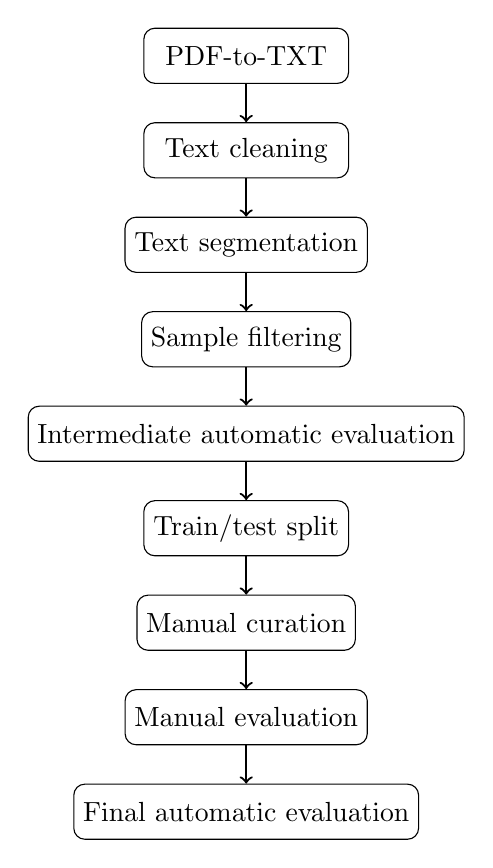
\begin{tikzpicture}[
    node distance=1.2cm,
    every node/.style={draw, rectangle, rounded corners, align=center, minimum width=2.6cm, minimum height=0.7cm},
    arrow/.style={->, thick}
]

\node (pdf) {PDF-to-TXT};
\node (clean) [below of=pdf] {Text cleaning};
\node (seg) [below of=clean] {Text segmentation};
\node (filter) [below of=seg] {Sample filtering};
\node (eval) [below of=filter] {Intermediate automatic evaluation};
\node (split) [below of=eval] {Train/test split};
\node (curation) [below of=split] {Manual curation};
\node (manualeval) [below of=curation] {Manual evaluation};
\node (finaleval) [below of=manualeval] {Final automatic evaluation};

\draw[arrow] (pdf) -- (clean);
\draw[arrow] (clean) -- (seg);
\draw[arrow] (seg) -- (filter);
\draw[arrow] (filter) -- (eval);
\draw[arrow] (eval) -- (split);
\draw[arrow] (split) -- (curation);
\draw[arrow] (curation) -- (manualeval);
\draw[arrow] (manualeval) -- (finaleval);

\end{tikzpicture}
}
\centering
\vspace{0.4cm}
\caption{Overview of the dataset construction pipeline.}
\label{fig:pipeline}
\end{figure}

\clearpage


\subsection{PDF-to-TXT}

PDF24 \citep{pdf24} was employed to convert each of the clinical guidebooks in PDF format into TXT format. This conversion step was necessary to enable easier textual processing. Although this introduces minor formatting noise (e.g. line breaks, headers, and pagination artifacts), these issues are addressed below in the cleaning stage.

\subsection{Text cleaning}

Each line extracted from the TXT files is normalized using a dedicated cleaning function. The function performs the following operations:

\vspace{-0.1cm}

\begin{itemize}
    \item Initial whitespace stripping.
    \vspace{-0.2cm}
    \item Bullet-like character removal: \{\textbullet{}, $\bullet$, \texttt{-}, \texttt{*}\}.
    \vspace{-0.2cm}
    % \item Removes LaTeX-style bullet markers (e.g., \texttt{\textbackslash bullet} and variants such as \texttt{\$\textbackslash bullet\$}) when they appear at the beginning of a line.
    \item Final whitespace stripping.
\end{itemize}

\vspace{-0.1cm}

This step is intended to ensure that the text segmentation operates on uniform textual units, thereby reducing noise introduced by PDF extraction artifacts.

\subsection{Text segmentation}

% The core of the pipeline is a rule-based segmentation system built using regular expressions. The text is processed sequentially line by line, and each line is assigned to a specific structural component based on pattern matching.

% The segmentation logic identifies the following input elements:

% \begin{itemize}
%     \item \textbf{topic}: detected using headers such as \textit{Pregunta}, \textit{Pregunta para responder}, or \textit{Subpregunta}, and accumulated until a \textit{Contexto} marker.

%     \item \textbf{question}: identified via patterns such as \texttt{a)}, marking the start of a new QA instance; previous samples are flushed upon detection.

%     \item \textbf{subquestion}: identified via patterns such as \texttt{a.1.}, and treated as optional structure within a question.

% \end{itemize}

% The segmentation logic identifies the following output elements:

% \begin{itemize}

%     \item \textbf{judgement}: triggered by \textit{“Juicio:”}, introducing the concise clinical answer.

%     \item \textbf{evidence}: triggered by \textit{“Evidencia procedente de la investigación:”}, introducing supporting textual evidence.

%     \item \textbf{considerations}: triggered by \textit{“Consideraciones adicionales:”} or \textit{“Información adicional:”}, capturing optional interpretative content.
% \end{itemize}




% Each output element is activated by a corresponding keyword trigger and then accumulates lines until a new section is detected. At each transition point (new question or subquestion), the accumulated data is stored as a structured row in a dataset. This design allows the reconstruction of hierarchical document structure (topic $\rightarrow$ question $\rightarrow$ subquestion $\rightarrow$ answers) from flat text.


The core of the pipeline is a rule-based text segmentation built using regular expressions. The text is processed sequentially, assigning each line to a structural component via pattern matching. The segmentation logic is composed of the following patterns to identify input features (\autoref{tab:input_triggers}) and output features (\autoref{tab:output_triggers}):

\begin{table}[H]
\centering
\small
\begin{tabular}{l|l|c}
\toprule
\textbf{Input feature} & \textbf{Patterns} & \textbf{e.g.} \\
\midrule
\textit{topic} & After "Pregunta" \\
      & After "Pregunta para responder" \\
      & After "Subpregunta" \\
      & Before "Contexto" \\
\midrule
\textit{question} & \texttt{\textasciicircum[a-z])} & \texttt{a)}  \\
\midrule
\textit{subquestion} & \texttt{\textasciicircum[a-z]\textbackslash.\textbackslash d+\textbackslash.} & \texttt{a.1.} \\
\bottomrule
\end{tabular}
\caption{Text segmentation patterns for input features.}
\label{tab:input_triggers}
\end{table}

% The segmentation logic identifies the following output elements:

\vspace{-0.2cm}

\begin{table}[H]
\centering
\small
\begin{tabular}{l|l}
\toprule
\textbf{Output feature} & \textbf{Patterns} \\
\midrule
\textit{judgement} & After "Juicio:" \\
\midrule
\textit{evidence} & After "Evidencia procedente de la \\
 &  investigación:" \\
 \midrule
\textit{considerations} & After "Consideraciones adicionales:" \\
               & After "Información adicional:" \\
\bottomrule
\end{tabular}
\caption{Text segmentation patterns for output features.}
\label{tab:output_triggers}
\end{table}

% Each structural element is identified via rule-based triggers and, when applicable, accumulates text until a new section is detected. 
Input features are derived from header and pattern-based markers, which define sample boundaries and control when instances are flushed. Output features are activated by keyword triggers and accumulate text until the trigger of the next feature. This mechanism enables reconstruction of a hierarchical structure (\textit{topic} → \textit{question} → \textit{subquestion} → \textit{answers}) from flat text.

% Each output element is feature by a corresponding keyword trigger and then accumulates lines until a new section is detected. At each transition point (new question or subquestion), the accumulated data is stored as a structured row in the dataset. This design allows the reconstruction of hierarchical document structure (topic $\rightarrow$ question $\rightarrow$ subquestion $\rightarrow$ answers) from flat text.

\subsection{Sample filtering}

After extraction, a filtering step was applied to remove noisy samples. In particular, 70 instances in the dataset contain only placeholder references in the \textit{evidence} feature: \textit{Ver apartado anterior} ("See previous section") / \textit{Ver apartados anteriores} ("See previous sections").

These cases were removed because they do not provide any bibliographical source, but instead refer to previous \textit{evidence} cells. Keeping these placeholder instances would imply associating a single bibliographical source to several clinical questions, which may blur the semantic distance among different QA instances. In fact, a short experiment I conducted with this dataset shows that RAG performance improves by 2.4\% when such instances are removed:

\begin{table}[H]
\centering
\begin{tabular}{lccc}
\toprule
\textbf{Data type} & \textbf{Unfiltered} & \textbf{Filtered} & \textbf{$\Delta$} \\
\midrule
judgement        & 84.5 & 85.3 & +0.8 \\
evidence         & 81.0 & 81.8 & +0.8 \\
considerations   & 79.7 & 85.2 & \textbf{+5.5} \\
overall & 81.7 & 84.1 & \textbf{+2.4} \\
\bottomrule
\end{tabular}
\caption{Cosine similarity (F1) results with and without sample filtering. Source: \url{https://github.com/iker-gutierrez/SNS-RAG-model-v1}.}
\label{tab:cosine_results}
\end{table}
 
 % eeping them would introduce noise in downstream applications such as retrieval-augmented generation and supervised training, where alignment between questions and their supporting evidence is essential.

% They cannot be reliably used for retrieval purposes, since the retriever will find repeated \textit{evidence} cells and will find it harder to distinguish between bibliographical sources.

% Additional filtering ensures that rows with missing mandatory fields (\textit{guidebook}, \textit{topic}, \textit{question}, \textit{judgement}, \textit{evidence}) are excluded from the final dataset.



\subsection{Intermediate automatic evaluation}

An intermediate quality check was performed to measure structural consistency. The presence rates of optional features are shown in \autoref{tab:intermediate_optional}. \textit{Subquestions} are infrequent, whereas \textit{considerations} are present in the majority of samples.

\vspace{-0.1cm}

\begin{table}[H]
\centering
\begin{tabular}{lc}
\toprule
\textbf{Feature} & \textbf{Non-empty cells (\%)} \\
\midrule
\textit{subquestion} & 4.51 \\
\textit{considerations} & 64.85 \\
\bottomrule
\end{tabular}
\caption{Presence rates of optional features in the intermediate dataset.}
\label{tab:intermediate_optional}
\end{table}

More important than quantifying optional features is verifying whether all cells of mandatory features are non-empty. \autoref{tab:intermediate_completeness} shows that the extraction pipeline achieves near-complete presence rates for mandatory features, with noise affecting the \textit{judgement} and \textit{evidence} features.

\begin{table}[H]
\centering
\begin{tabular}{lc}
\toprule
\textbf{Feature} & \textbf{Non-empty cells (\%)} \\
\midrule
\textit{guidebook} & 100.00 \\
\textit{topic} & 100.00 \\
\textit{question} & 100.00 \\
\textit{judgement} & \textbf{99.91} \\
\textit{evidence} & \textbf{98.97} \\
\bottomrule
\end{tabular}
\caption{Presence rates of mandatory features in the intermediate dataset.}
\label{tab:intermediate_completeness}
\end{table}

11 mandatory cells from \textit{judgement} and \textit{evidence} columns were identified as empty. The implemented regular expressions did not properly catch the text segmentations for these instances. These samples were flagged for inspection and correction during the manual curation stage.
% These correspond to the following indices: \texttt{[38, 506, 869, 967, 979, 980, 989, 990, 999, 1000, 1009]}.

\subsection{Train/test split}

The dataset is divided into train and test sets with a 80\%-20\% split, stratified by \textit{guidebook}. Stratification preserves the original proportions of samples per guidebook and accordingly ensures there will be samples from all guidebooks in both sets. The split is performed at the sample level, retaining the dataset structure across both sets. \autoref{tab:train_test_split} shows the data distribution:
% As shown in  , this results in 851 training samples and 213 test samples.

\begin{table}[H]
\centering
\begin{tabular}{lrr}
\toprule
\textbf{Set} & \textbf{Samples} & \textbf{Percentage} \\
\midrule
Train & 851 & 80\% \\
Test  & 213 & 20\% \\
\bottomrule
\end{tabular}
\caption{Train/test split of the SNS-1064 dataset.}
\label{tab:train_test_split}
\end{table}



\subsection{Manual curation}

For a reliable evaluation of clinical RAG models, the test set should be noiseless. Hence, a manual curation process was performed on the entire test set (\fontsize{10pt}{11pt}\texttt{test\_df}\normalsize). However, the training set  (\fontsize{10pt}{11pt}\texttt{train\_df}\normalsize) was only partially inspected, as noise is less critical in training data and full manual curation would be highly time-consuming.

The goal of the manual curation step was to fix segmentation errors and guarantee that each sample correctly reflects the intended structure of the source documents.

\subsection{Manual evaluation}

The manual curation concomitantly allowed for a qualitative evaluation of the rule-based pipeline. Overall, the regular expressions for text cleaning and segmentation performed effectively. The majority of samples were correctly structured, but a couple of systematic errors were identified:

\begin{itemize}
    \item Page headers and footers occasionally remained in the extracted text due to limitations of the PDF-to-TXT conversion.
    \item In some cases, the \textit{considerations} information was included in the \textit{evidence} feature, evincing that the regex for \textit{considerations} did not catch all text segmentations properly. However, this is a minor issue, since the \textit{evidence} and \textit{considerations} features do not differ substantially. Both are output features that explain the \textit{judgement}.
\end{itemize}

% Moreover, please recall that the train set was only partially curated. Therefore, some noise is expected in the training data.


\subsection{Final automatic evaluation}

After manual curation of the dataset, a final automatic evaluation was conducted to verify that all corrections had been successfully incorporated.

Results show a fully consistent dataset with respect to mandatory features. No incomplete samples were detected after curation, confirming the effectiveness of the manual review process.

\begin{table}[H]
\centering
\begin{tabular}{lc}
\toprule
\textbf{Feature} & \textbf{Non-empty cells (\%)} \\
\midrule
\textit{guidebook} & 100.00 \\
\textit{topic} & 100.00 \\
\textit{question} & 100.00 \\
\textit{judgement} & \textbf{100.00} \\
\textit{evidence} & \textbf{100.00} \\
\bottomrule
\end{tabular}
\caption{Presence rates of mandatory features after manual curation.}
\label{tab:final_completeness}
\end{table}

Regarding optional features, \autoref{tab:final_optional} compares their distribution before and after manual curation. The results show that \textit{subquestion} remains virtually unchanged (+0.10), while \textit{considerations} exhibits a more notable increase (+1.50). 
% Overall, these variations are limited, indicating that manual curation primarily addressed structural issues without substantially modifying annotation frequencies.

\begin{table}[H]
\centering
\begin{tabular}{lcc}
\toprule
\textbf{Feature} & \textbf{Non-empty cells (\%)} & $\Delta$  \\
\midrule
\textit{subquestion} & 4.61 & +0.10 \\
\textit{considerations} & 66.35 & \textbf{+1.50} \\
\bottomrule
\end{tabular}
\caption{Presence rates of optional features after manual curation.}
\label{tab:final_optional}
\end{table}

Overall, manual curation improved structural segmentation without altering the quality of the expert annotations.

% The stability of these values indicates that manual curation focused exclusively on structural corrections , preserving the original distribution of optional annotations.


\section{Applicability to RAG-based clinical QA}

The SNS-1064 dataset is designed to support RAG systems in the clinical domain. By explicitly separating answers (\fontsize{10pt}{11pt}\texttt{judgement} \normalsize column) from scientific evidence (\fontsize{10pt}{11pt}\texttt{evidence} \normalsize column) and additional considerations (\fontsize{10pt}{11pt}\texttt{considerations} \normalsize column), the dataset enables:

\begin{itemize}
    \item Improved grounding of generated answers in clinical text.
    \item Better retrieval alignment between questions and evidence passages.
    \item Enhanced interpretability through structured reasoning components.
\end{itemize}

This structure is particularly relevant for high-stakes domains such as healthcare, where factuality, explainability, and traceability of model outputs are essential.

\section{Conclusion}

This paper presented the SNS-1064 dataset for RAG-based clinical QA tasks in Spanish. The construction pipeline transforms PDF clinical guidebooks into structured instances composed of: question + answer + evidence. Future work may include dataset expansion, more powerful quality evaluation methods, and curation of the entire training set by either manual or automatic means.
% automatic quality validation, and integration with large language model evaluation frameworks.



\bibliography{bibliography}
\bibliographystyle{acl_natbib}

\end{document}